\documentclass{article}
\usepackage{amssymb}
\usepackage{changepage}
\usepackage[fleqn]{amsmath}
\usepackage{gensymb}
\usepackage{cancel}
\usepackage{tkz-euclide}
\usepackage{graphicx}
\title{Hooke's Law Lab}
\author{SPH-4UI - Tristan Simpson}

\begin{document}
\maketitle

\vspace{0.5cm}
\hrule
\vspace{0.5cm}
\section*{Purpose}
The purpose of this lab was to determine the spring constant between different masses.
This was done by utilizing the formula $F_{s} = \frac{x}{k}$

\section*{Materials}
\begin{enumerate}
    \item {\textbf{One of Each} 100g, 150g, 200g, 500g, 700g, 1000g Weights.}
    \item {\textbf{One} Wooden Apparatus.}
    \item {\textbf{One} Spring.}
    \item {\textbf{One} Meter-stick.}
    \item {\textbf{One} Clamp.}
\end{enumerate}

\section*{Procedure}
\begin{enumerate}
    \item {The wooden apparatus was clamped to the table such that the nail on it's end was facing downwards.}
    \item {The spring was hooked to the nail on the wooden apparatus.}
    \item {The initial stretch of the spring was measured and documented.}
    \item {The smallest weight was attached to the bottom of the hanging spring.}
    \item {As the weight comes to a rest, measure the distance from the top of the spring to it's bottom and document the result.}
    \item {Repeat the above steps for the remaining weights.}
\end{enumerate}\leavevmode

\section*{Observations}
\textit{Data provided by Ibrahim Khan}\newline
The initial height of the spring was 52.3cm. This is used in finding $x$ with $h\prime - h$.
The below table exhibits the groups observations during the experiment. Using this data we can calculate the spring constant between the different masses.\newline
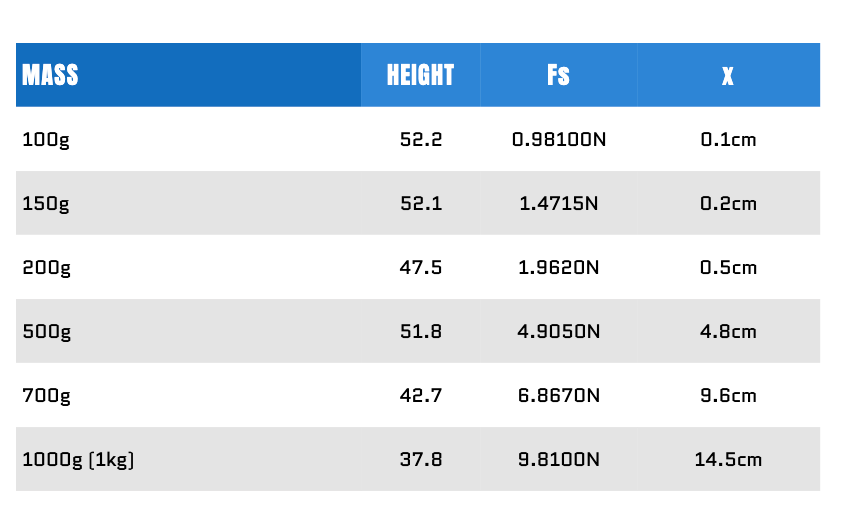
\includegraphics[scale=0.5]{./images/data_table.png}
\section*{Calculations}
\noindent To solve for the spring constant of this experiment a random row of data from the observations table was substituted into the formula: $F_{s} = \frac{x}{k}$
\newline

\noindent\textbf{Result:} \\
\begin{adjustwidth}{0.5cm}{0pt}
    $F_{s} = \frac{x}{k}$ \\\\
    $\therefore k = \frac{F_{s}}{x} = \frac{4.9050}{0.04800} \approx 102\frac{N}{m}$
\end{adjustwidth}

\section*{Sources of Error}
\subsection*{Errors}
\begin{enumerate}
    \item {The spring was overstretched and worn out.}
    \item {The spring swayed, giving it components.}
    \item {The spring was rusty.}
\end{enumerate}
\subsection*{Solutions}
\begin{enumerate}
    \item {This problem could be resolved by using a new spring.}
    \item {This problem could be resolved by having an object hold the spring inplace.}
    \item {This problem could be resolved by using a new spring.}
\end{enumerate}\leavevmode

\section*{Conclusion}
By the conclusion of this lab it was determined that the spring constant was approximately $102\frac{N}{m}$.
The accuracy of this lab could have been improved by using multiple rows of data for determining the spring constant instead of just one.

\section*{Synthesis}
The learnings from this lab can be applied to numerous real-world scenarios.
First, having a direct application to the experiment is the force exterted on a stapler's spring. Inside each stapler lies a spring that compressed and decompresses when it's user pushes on it.
Secondly, similar to the stapler is a trampoline. Unlike the stapler the springs in a trampoline are far stronger and do not compress/decompress as easily. This is to compensate for the jumpers mass.
Finally, also similar to the above implications are the springs inside a keyboard.
\end{document}